% !TEX TS-program = xelatex
% !TEX encoding = UTF-8

% This is a simple template for a XeLaTeX document using the "article" class,
% with the fontspec package to easily select fonts.

\documentclass[12pt]{article} % use larger type; default would be 10pt

\usepackage[height=9.5in,a4paper,hmargin={3cm,0.8in},vmargin=0.75in,left=1.0in]{geometry}                % See geometry.pdf to learn the layout options. There are lots.

%\usepackage[tmargin=1in,bmargin=1in,lmargin=1.25in,rmargin=1.25in]{geometry}
\usepackage{fontspec}
\usepackage{xcolor}
\usepackage{titlesec}
\usepackage{graphicx} % support the \includegraphics command and options
\usepackage{xunicode} % Unicode support for LaTeX character names (accents, European chars, etc)
\usepackage{xltxtra} % Extra customizations for XeLaTeX
\usepackage{textgreek} % Use Greek Letters without Math Package
\usepackage{amsmath} % for the Matrix


\newcommand{\HRule}{\rule{\linewidth}{0.5mm}}

\defaultfontfeatures{Ligatures=TeX}
\defaultfontfeatures{Mapping=tex-text} % to support TeX conventions like ``---''

\setmainfont{Arial} % set the main body font (\textrm), assumes Charis SIL is installed
\setsansfont{Times}
\setmonofont{Monaco}

% Define light and dark Microsoft blue colours
\definecolor{Black}{rgb}{0.0 0.0 0.0}

% Define a new fontfamily for the subsubsection font
% Don't use \fontspec directly to change the font
%\newfontfamily\sectionfont[Color=MSLightBlue]{Helvetica}
% Set formats for each heading level

\titleformat*{\section}{\large\bfseries\sffamily\color{Black}}
\titleformat*{\subsection}{\small\bfseries\sffamily\color{Black}}
\titleformat*{\subsubsection}{\small\bfseries\sffamily\color{black}}

\begin{document}

%\begin{titlepage}
\begin{center}
% Upper part of the page
\textsc{\huge Development Notes for DREAM3D}\\[1.5cm]
\textsc{\large DREAM3D Development Team\\
Email: dream3d@bluequartz.net}\\[1.5cm]
%\vfill
% Bottom of the page
%{\large \today}
\end{center}
%\end{titlepage}

%----------------------------------------------------------
% Set Table of Contents
%----------------------------------------------------------
%\clearemptydoublepage
\pagenumbering{roman}
%\tableofcontents
%\listoffigures
%\listoftables
%\pagenumbering{arabic}
%\newpage
\section{Intro (or why this file)}
  This is just a dumping ground for ideas that we are working on.

\section{Image Processing Introduction}


Images that are imported into DREAM3D should probably be segmented using a preprocessing tool as there are currently no effective tools to do the segmentation in DREAM3D itself. If your images are already preprocessed so that they are segmented into specific regions DREAM3D may be able to work with the image data and give you meaningful results. There are probably 3 categories of images that DREAM3D can handle with some modifications to current filters.


\begin{itemize}
\item The regions of the image that represent a phase or grain each have a unique identifier such as a gray scale value or unique RGB value.\ref{figure:Type1}
\item There are regions that represent grains where each region has a unique identifier but there are multiple regions with the same identifier. \ref{figure:Type2}
\item Each Grain is traced out via a another pixel identifier so that grain boundaries are "black" and each grain is "white". \ref{figure:Type3}
\end{itemize}

DREAM3D will need to implement filters with algorithms that can work with these cases and bring a consistent grain numbering to the imported volume which is important for things like the statistics and surface meshing routines.

\begin{figure}[htbp]
\begin{center}
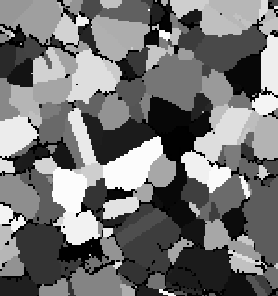
\includegraphics[width=2.5in]{Type1.png}
\caption{}
\label{figure:Type1}
\end{center}
\end{figure}

\begin{figure}[htbp]
\begin{center}
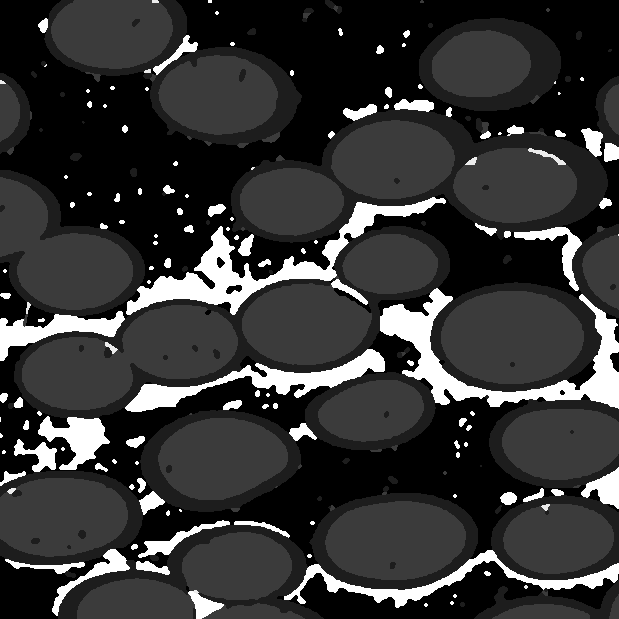
\includegraphics[width=2.5in]{Type2.png}
\caption{}
\label{figure:Type2}
\end{center}
\end{figure}



\begin{figure}[htbp]
\begin{center}
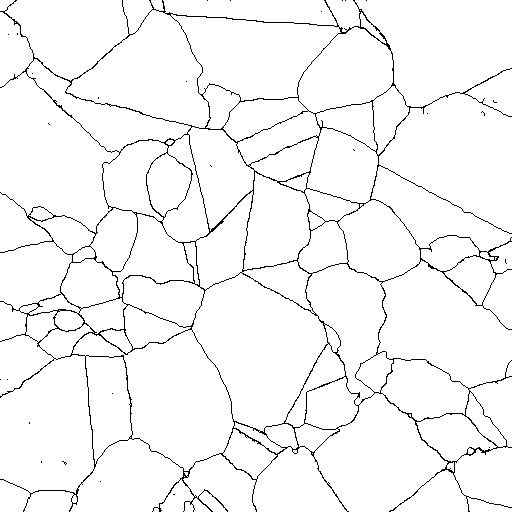
\includegraphics[width=2.5in]{Type3.png}
\caption{}
\label{figure:Type3}
\end{center}
\end{figure}



\section{Xdmf File}
  Explain what the Xdmf file is and how it can be used.

\section{Grain Face Curvature Updates}
	Add user specified option to use the Normals for the fitting routine or NOT use the normals. Update documentation with some of the equations for the curve fitting portion of the calculation. Use LATEX to generate the equation images.

\section{Surface Mesh Output}
	Figure out how to write an XDMF file that has a non-conformal mesh, ie, 2 triangles so the user can extract single grains

\section{Export Binary File}
  We should be able to export any of the arrays into a raw binary file for import into other analysis programs. 
  
\section{Parallelize Synthetic Generators}
   Initial threading of PackPrimaryGrains was performed using the parallel\_for() construct from the Threading Building Blocks (TBB) package. We are achieving a decent speed up on multi-core hardware. We could probably realize more speed ups just using more efficient algorithms.
   
   Thread up the InsertPrecipitates code. It is essentially the same as the PackPrimaryGrains code.

\section{DREAM3D Reader}
 Allow the data being read into DREAM3D to be appended to the data container if it does not already exist. Currently when reading the DREAM3D file the entire data containers are wiped out. If the same array is read then the user could have the option to over write the existing array with the data from the file. This opens up the ability to append files together or get data from several different sources.  
 
\section{PipelineRunner Program}
  This program should be able to use as an input a Pipeline text file saved from the GUI. The requires the use of Qt libraries to read the .ini style file and the sometimes specially encoded QVariant class within the .ini file. In order to do this I tried linking against the generated widgets library and simply invoking a PipelineBuilderWidget class but Qt borked on that saying that we needed to have a QApplication running which is will probably start popping up QWidgets on the screen which is not really what we want.\\
  
  
 One idea was to further break apart the QFilterWidget and to have something like a QFilterProxy object that holds the values from the gui but before the gui stuffs those values into the actual Filter instance object. The QFilterProxy would simply inherit from the QObject class so that we can use the QObject's property system which reading from the QSettings file is going to require. Either that or we generate a QFilterProxy file for each filter like we do for the QFilterWidgets which will add to the amount of code that needs to be compiled but should work in the long run.

\section{GUI Enhancements}
   Be able to "right click" on a "Favorite" filter and Delete/Rename/export it


\section{Image Filters}
   Now that we can import an image we should create a filter that can export a volume as a stack of images and do the coloring based on one of the arrays in the Cell Data like grain Ids or IPF Colors.

\section{Image Processing Library Addition}
   We need to probably include ITK, VTK, OpenCV or some other image processing library in DREAM3D if possible rather than writing each filter individually. Lets ride on the coat-tails of someone else.

   
\section{Execute External Program Filter}
	We should be able to write a filter that takes the location of a program and the arguments to that program and then DREAM3D will execute that program with the given arguments. Pair this up with the export/import of binary data or images and you now have a way to do somethings in DREAM3D, fork to MatLab or IDL and the bring the output data back into DREAM3D. If enough time we given I would use the Widget for "Comparison" Threshold filter so clicking the "+" button would add another argument. This may make it easier for the user to group their arguments together if the argument list is very long. The preflight would make sure the program is available and maybe show the output from the program?

 
   
\section{Voxel Dimensions During Pipeline}
What about adding this information to the QFilterWidget and a "pop-up" window or "disclosable" piece of information?

  
\section{Python Bindings}
  We need to figure out if it is possible to auto generate python bindings for DREAM3D. This would come in very handy for writing python scripts for processing of data and using other python frameworks like PyQt and Image processing libraries written in python.
  
\section{Documentation}
  As always the documentation for each filter is woefully underdone.
  
\section{Tutorials}
  We need more tutorials on the following:
  \begin{itemize}
  \item Synthetic Structures with all sorts of different types displayed and generated
  \item Importing more data types
  \item Meshing and Smoothing a volume
  \item cleaning up a volume, ie, getting rid of "bad" data voxels.
  \item Concrete examples of each filter and the before and after with images. (THIS IS WHERE AN IMAGE EXPORT filter would come in handy as one could almost automate some of this)
  \item 
  \end{itemize}


\section{Updated Build Documentation}
  Prebuilt binaries for the DREAM3D SDK might be nice if possible.
  
\section{Developer Opportunities}
  \begin{itemize}
  \item FEM File formats
  \item Improved Meshing (Surface and Volume)
  \item Image processing Filters
  \item Python Bindings
  \end{itemize}

   
\end{document}